\chapter{Theoretical Foundation} \label{ch:theoretical_foundation}

In order to investigate the phenomenon of in-between instances (IBIs) and the potential limitations of autoencoders in capturing them, it is essential to first establish a solid theoretical grounding. This chapter introduces these two central conceptual frameworks that underpin this thesis.

\section{Autoencoder}

Autoencoders are a class of artificial neural networks designed to learn efficient, compressed representations of input data in an unsupervised manner. Originally introduced by Rumelhart et al. (1987) \cite{Rumelhart86}, autoencoders have since become a cornerstone of deep learning-based representation learning, particularly for tasks involving dimensionality reduction, data compression, and generative modeling. Their key strength lies in their ability to learn latent features that capture the essential structure of the data without requiring labeled examples.

\subsection{Architecture}

An autoencoder is fundamentally a feedforward neural network comprising three main layers: the input layer, a hidden representation (or code), and the output layer [\cite{Goodfellow16}, \cite{Berahmand24}]. The encoder-decoder architecture is presented in Figure \ref{fig:autoencoder}. The encoder maps the input data 
$\mathbf{x} \in \mathbb{R}^n$ 
to a latent space 
$\mathbf{h} \in \mathbb{R}^m$, 
where typically $m < n$. This mapping is performed by a function 
$f_{\theta}(\cdot)$, 
parameterized by weights and biases $\theta$, such that 
$\mathbf{h} = f_{\theta}(\mathbf{x})$. 
The decoder performs the inverse operation, mapping the latent representation back to the reconstructed input 
$\hat{\mathbf{x}}$, 
using a function 
$g_{\phi}(\cdot)$, 
parameterized by $\phi$, such that 
$\hat{\mathbf{x}} = g_{\phi}(\mathbf{h})$.

\begin{figure}[ht]
  \centering
  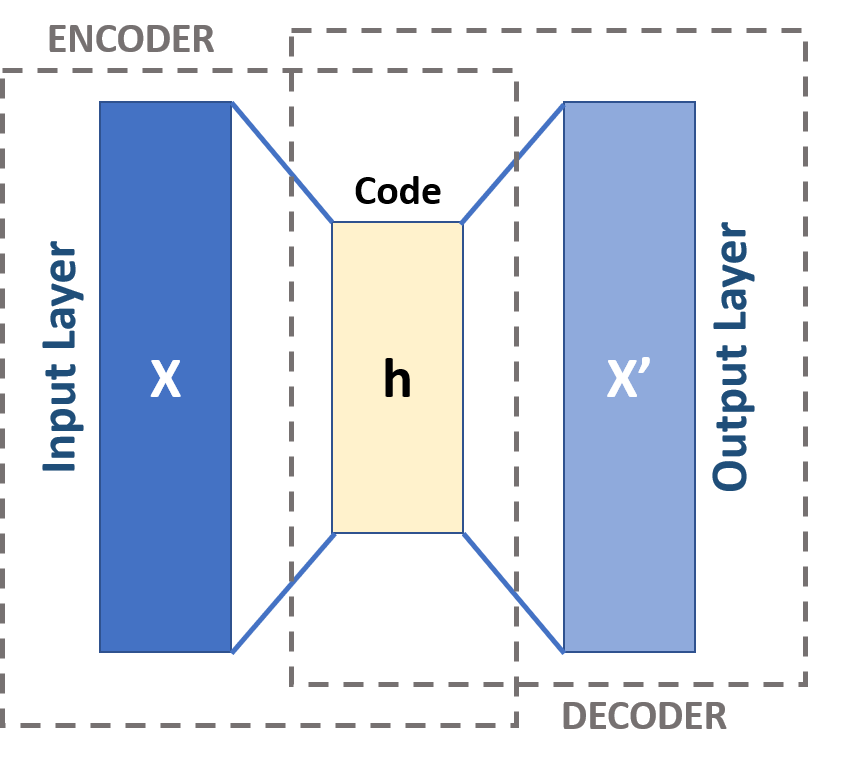
\includegraphics[width=0.50\textwidth]{images/Autoencoder_schema.png}
  \caption{The architecture of an standard autoencoder. Adapted from \url{https://upload.wikimedia.org/wikipedia/commons/3/37/Autoencoder_schema.png}}
  \label{fig:autoencoder}
\end{figure}

Typically, both $f_{\theta}$ and $g_{\phi}$ are implemented using neural network layers, often fully connected (dense) layers for tabular data or convolutional layers for image data. The activation functions used in the encoder and decoder vary by application but often include rectified linear units (ReLU) \cite{ReLU}, sigmoid, or tanh functions.

The bottleneck layer forces the model to learn the most salient features of the data by constraining the capacity of the network. This compression is critical for enabling the autoencoder to generalize rather than simply memorizing the input data.

\subsection{Training}

Training an autoencoder involves optimizing the parameters $\theta$ and $\phi$ to minimize the discrepancy between the input $\mathbf{x}$ and its reconstruction $\hat{\mathbf{x}}$. This discrepancy is typically measured using a reconstruction loss function, such as the mean squared error (MSE) for continuous data. This objective is minimized using stochastic gradient descent (SGD) or its variants such as Adam \cite{Adam}, RMSProp \cite{RMSProp}, or Adagrad \cite{Adagrad}. The gradients are computed via backpropagation, which adjusts the weights in both the encoder and decoder networks simultaneously. Proper number and size of layers, the learning rate, the loss function, and the regularization are crucial for stable and efficient training \cite{Berahmand24}.

\subsection{Variants}

Over time, numerous variants of the basic autoencoder have been proposed to overcome its limitations and enhance its representational power. One of the most influential extensions is the \textbf{denoising autoencoder} [\cite{Vincent08}, \cite{Goodfellow16}], which aims to learn robust features by reconstructing clean input from a corrupted version. By forcing the network to recover original data from noisy inputs, the model learns more meaningful representations that are invariant to small perturbations.

Another popular modification is the \textbf{sparse autoencoder}, which introduces a sparsity constraint on the latent representation. This is commonly implemented by adding a regularization term that penalizes activation levels across neurons in the bottleneck layer, encouraging the network to activate only a small subset of neurons for any given input [\cite{Ng11}, \cite{Goodfellow16}]. Such sparsity tends to produce more interpretable features and has been linked to mechanisms in biological neural systems.

A more sophisticated probabilistic framework is introduced in the \textbf{variational autoencoder (VAE)}, proposed by Kingma and Welling (2013) [\cite{Kingma13}, \cite{Bank21}]. Unlike classical autoencoders that learn a deterministic mapping to the latent space, VAEs model the latent variables as probability distributions. The encoder outputs parameters of a distribution (usually Gaussian), and the decoder generates data by sampling from this distribution. Training is achieved by maximizing the evidence lower bound (ELBO), which balances the reconstruction loss and a Kullback-Leibler (KL) divergence term that regularizes the latent distribution toward a prior, typically standard normal. This approach enables both principled generative modeling and smooth interpolation in latent space.

Further developments include \textbf{adversarial autoencoders} \cite{Makhzani16}, which incorporate an adversarial loss similar to generative adversarial networks (GANs) to shape the distribution of the latent space. Other variations include convolutional autoencoders for spatial data, recurrent or sequence-to-sequence autoencoders for temporal data, and \textbf{contractive autoencoders} that penalize the Jacobian of the encoder to enforce local invariance [\cite{Rifai11}, \cite{Goodfellow16}].

\subsection{Applications}

Autoencoders have found extensive use across a wide range of domains, owing to their ability to learn compact and informative representations of data without requiring labeled supervision. One of their earliest and most prominent applications is in \textbf{dimensionality reduction} \cite{Goodfellow16}, where they serve as nonlinear generalizations of classical techniques such as principal component analysis (PCA). While PCA can only capture linear structures, autoencoders are capable of modeling complex, nonlinear manifolds in high-dimensional input spaces \cite{Hinton06}. This capability makes them particularly effective for visualizing high-dimensional datasets such as image or genomic data, where structure and variation are not easily captured by linear projections.

Autoencoders are also widely utilized in \textbf{anomaly detection} tasks. When trained exclusively on data that are representative of a “normal” class, the model learns to reconstruct these inputs accurately. Anomalous or out-of-distribution data, which deviate significantly from the training distribution, typically result in poor reconstructions and thus higher reconstruction error [\cite{Sakurada14}, \cite{Bank21}]. This principle has been successfully applied in diverse fields including network intrusion detection, manufacturing quality assurance, and medical diagnostics.

In the realm of \textbf{denoising}, autoencoders have been used to remove noise and corruption from data. Denoising autoencoders \cite{Vincent08} are trained to recover clean inputs from deliberately perturbed versions, thereby learning noise-invariant features that generalize better to unseen data. This approach has proven especially useful in image and audio preprocessing tasks.

Another influential application of autoencoders lies in \textbf{generative modeling}. Variational autoencoders (VAEs), in particular, provide a principled probabilistic framework for generating new data samples by sampling from the learned latent distribution [\cite{Kingma13}, \cite{Bank21}]. This has led to applications in synthetic data generation, drug discovery, and creative domains such as music and art synthesis. The ability to interpolate and manipulate attributes in the latent space allows VAEs to perform meaningful transformations, such as morphing one face into another or altering specific attributes like lighting and expression.

\subsection{Limitations}

Despite their versatility, autoencoders are subject to several limitations that affect their performance and general applicability. A fundamental issue is their potential to \textbf{learn trivial identity mappings} when the architecture is unconstrained, especially if the bottleneck layer has equal or greater dimensionality than the input. In such cases, the autoencoder may merely memorize inputs without learning meaningful abstractions \cite{Goodfellow16}. This problem is mitigated by architectural constraints (such as an undercomplete representation) or regularization techniques (e.g., sparsity or noise), but it remains an inherent risk in their design.

A notable limitation of autoencoders lies in their \textbf{sensitivity to hyperparameter settings}, which can significantly affect model performance and generalizability \cite{Berahmand24}. Critical hyperparameters such as the dimensionality of the latent space, number of layers, learning rate, regularization strength, and activation functions must be carefully tuned, often through empirical trial and error or computationally expensive search procedures. Poor choices can lead to underfitting, overfitting, or convergence failures.

Another limitation concerns the \textbf{interpretability of learned features} \cite{Bengio14}. Unlike linear methods such as PCA, where each principal component can often be directly interpreted in terms of variance directions, the latent variables learned by standard autoencoders are typically entangled and lack semantic meaning. This makes it challenging to use the latent space for tasks that require transparency or explanation, such as decision support systems in healthcare.

\section{In-Between Instance}

Traditional data-mining paradigms typically categorize data points either as inliers, members of well-defined clusters, or as outliers, which deviate significantly and are often discarded. However, Kazempour et al. (2024) \cite{Kazempour24} identify a third, crucial class of elements: \textbf{in-between instances (IBIs)}. These objects do not cleanly fit into one cluster, nor do they belong to the noise category. Instead, they act as bridges, sharing properties of two or more clusters.

\subsection{Definition}

Kazempour et al. (2024) \cite{Kazempour24} formalizes in-between instances as follows: \\
\textit{Given a dataset \( X \in \mathbb{R}^{n \times d} \). Furthermore, given a partitioning $C = \{ C_1, \ldots, C_k \} \subseteq X$ and a set of outliers \( O \subseteq X \) where \( C \cap O = \emptyset \) and \( \{X\} = C \cup O \). An object \( o \in O \) is an in-between instance if it is:
\begin{itemize}
    \item[(a)] deviating mostly from the characteristics of clusters (groups) and
    \item[(b)] still exhibits some characteristics of at least two or more clusters.
\end{itemize}
This property manifests itself in the observation of an in-between instance being located between two or more clusters. Here the term \textbf{between} bares the semantic of an object being in proximity of two or more clusters, hence being potentially similar with respect to the characteristics of the clusters it is located in-between.}

Mathematically, an IBI is identified through a predicate function, or criteria, $\theta(o, C_i, C_j)$ that evaluates whether an object $o$ is in between clusters $C_i$ and $C_j$. This function is flexible and domain-specific. It may incorporate geometric properties, probabilistic affiliations, or angular relationships, depending on the chosen framework. Crucially, the IBI is not reducible to a fuzzy member of one cluster, as in soft clustering approaches, nor is it merely an outlier in the traditional sense. It occupies a third semantic and structural space that bridges categorical boundaries.

\subsection{Criteria}

Kazempour et al. (2024) \cite{Kazempour24} delineate three principal criteria, or predicate classes, by which IBIs may be recognized. Each is grounded in a different aspect of spatial or statistical analysis and is suited to different data geometries and interpretative goals.

\begin{figure}[htbp]
    \centering
    \begin{subfigure}[b]{0.475\textwidth}
        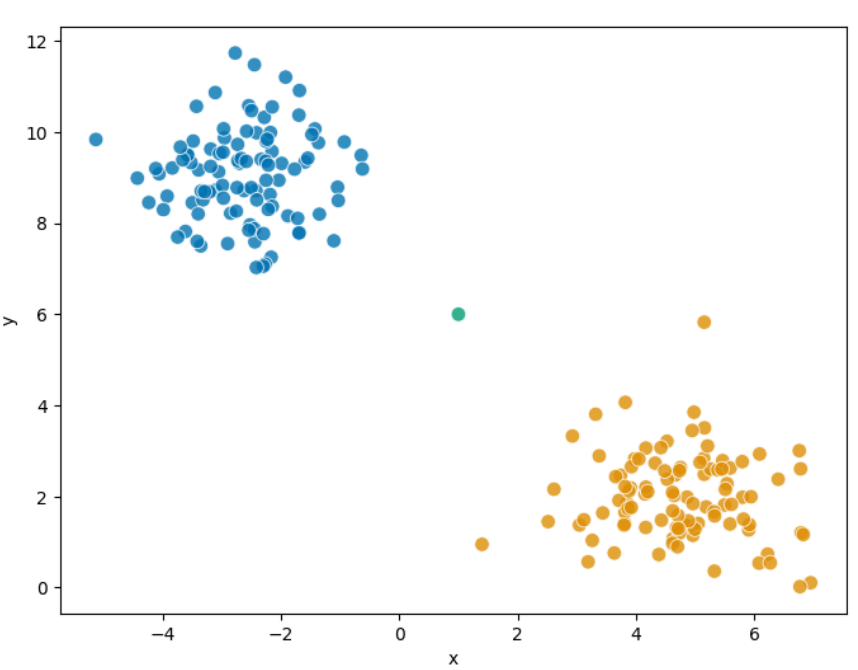
\includegraphics[width=\textwidth]{images/ibi_raw.png}
        \caption{Two clusters of data in blue and orange with an in-between instance in green.}
        \label{fig:ibi_raw}
    \end{subfigure}
    \hfill
    \begin{subfigure}[b]{0.475\textwidth}
        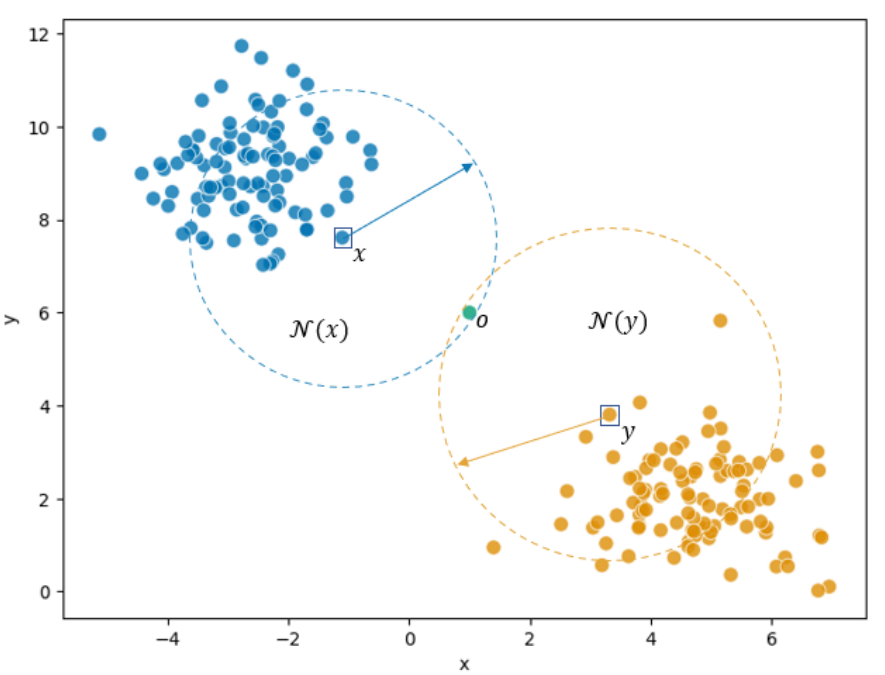
\includegraphics[width=\textwidth]{images/ibi_neighbor.png}
        \caption{Illustration of the neighborhood criterion for in-between instances.}
        \label{fig:ibi_neighbor}
    \end{subfigure}
    \vspace{0.5cm}
    \begin{subfigure}[b]{0.475\textwidth}
        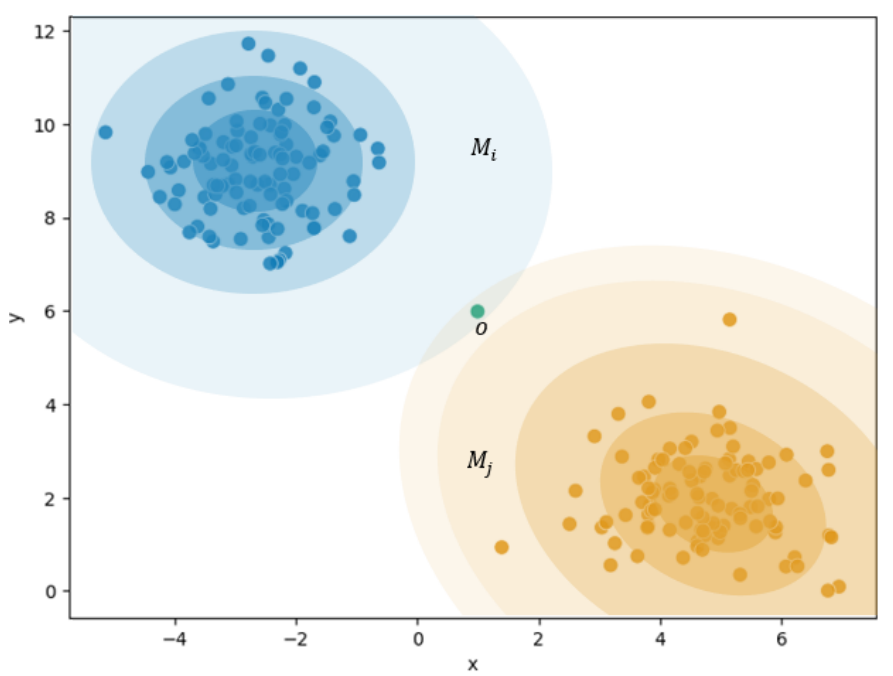
\includegraphics[width=\textwidth]{images/ibi_probability.png}
        \caption{Illustration of the class probability criterion for in-between instances.}
        \label{fig:ibi_probability}
    \end{subfigure}
    \hfill
    \begin{subfigure}[b]{0.475\textwidth}
        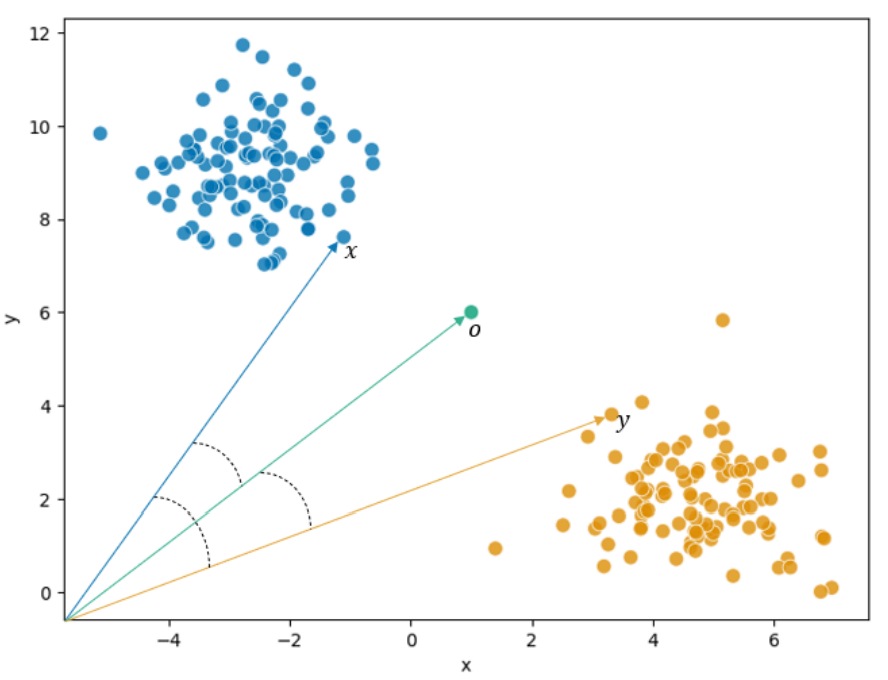
\includegraphics[width=\textwidth]{images/ibi_angle.png}
        \caption{ Illustration of the geometric criterion for in-between instances.}
        \label{fig:ibi_angle}
    \end{subfigure}
    \caption{In-between instances and its different criteria. Adapted from \cite{Kazempour24}}
    \label{fig:ibi}
\end{figure}

The \textbf{neighborhood criterion} (Figure \ref{fig:ibi_neighbor}) identifies IBIs based on local proximity. Here, an object is considered in-between if it resides within the spatial neighborhoods of at least two clusters, as determined by shared $k$-nearest neighbors or overlapping $\epsilon$-radius balls.

According to the \textbf{class probability criterion} (Figure \ref{fig:ibi_probability}), an object is an IBI if it has near-equal probabilities of belonging to at least two distinct clusters. This approach captures probabilistic ambiguity, which is especially useful in domains where uncertainty is intrinsic, such as medical diagnosis or probabilistic reasoning.

The \textbf{geometric criterion} (Figure \ref{fig:ibi_angle}) leverages vector relationships in high-dimensional space. An object is in-between if it lies directionally between representative points of two clusters. Formally, this is often framed in terms of the cosine similarity metric. An IBI, by this account, is positioned such that the angles between its vector representation and those of two cluster members are comparable, thereby confirming its intermediary status.

Each of these criteria reveals a different facet of in-betweenness and may be used independently or in combination to increase robustness and interpretability.

\subsection{Relationships to Clustering and Outlier Detection}

The concept of in-between instances reshapes traditional understandings of unsupervised learning by inserting a structurally distinct category between inliers and outliers. In classical clustering, objects are assigned to the cluster whose prototype or centroid they most closely resemble, often under assumptions of convexity or spatial separation. Outlier detection, by contrast, treats any point that deviates significantly from such groupings as anomalous, assuming it to be irrelevant noise or a rare event.

IBIs subvert this framework. They are outliers in the sense that they do not cleanly belong to any single cluster, but they are not statistical anomalies without meaning. Instead, they encode partial membership or blended features from multiple groups. This characteristic makes IBIs particularly valuable in complex, high-dimensional datasets where hybrid or transitional objects occur naturally. For example, in cultural analytics, an IBI might be a text that synthesizes themes from two distinct genres. In genomics, it might be a gene that functions across multiple pathways. In customer segmentation, an IBI could represent a consumer whose behavior aligns partially with multiple buyer personas.

Notably, IBIs are not captured by conventional clustering algorithms, including k-means \cite{kMeans} or DBSCAN \cite{DBSCAN}, nor by most standard outlier detectors like LOF (Local Outlier Factor) \cite{LOF}. These methods are not designed to detect shared affinities across cluster boundaries. Similarly, fuzzy clustering methods assign soft membership probabilities but do not explicitly highlight cases of balanced ambiguity or inter-cluster affinity. The IBI framework proposed by Kazempour et al. (2024) \cite{Kazempour24} fills this conceptual and methodological gap, proposing concepts to identify, quantify, and interpret these intermediate cases.
